\documentclass{article}

\usepackage{amsmath, amsthm, amssymb, amsfonts}
\usepackage{thmtools}
\usepackage{graphicx}
\usepackage{setspace}
\usepackage{geometry}
\usepackage{float}
\usepackage{hyperref}
\usepackage[utf8]{inputenc}
\usepackage[english]{babel}
\usepackage{framed}
\usepackage[dvipsnames]{xcolor}
\usepackage{tcolorbox}

\colorlet{LightGray}{White!90!Periwinkle}
\colorlet{LightOrange}{Orange!15}
\colorlet{LightGreen}{Green!15}

\newcommand{\HRule}[1]{\rule{\linewidth}{#1}}

\declaretheoremstyle[name=Theorem,]{thmsty}
\declaretheorem[style=thmsty,numberwithin=section]{theorem}
\tcolorboxenvironment{theorem}{colback=LightGray}

\declaretheoremstyle[name=Proposition,]{prosty}
\declaretheorem[style=prosty,numberlike=theorem]{proposition}
\tcolorboxenvironment{proposition}{colback=LightOrange}

\declaretheoremstyle[name=Principle,]{prcpsty}
\declaretheorem[style=prcpsty,numberlike=theorem]{principle}
\tcolorboxenvironment{principle}{colback=LightGreen}

\setstretch{1.2}
\geometry{
    textheight=9in,
    textwidth=5.5in,
    top=1in,
    headheight=12pt,
    headsep=25pt,
    footskip=30pt
}

% ------------------------------------------------------------------------------

\begin{document}

% ------------------------------------------------------------------------------
% Cover Page and ToC
% ------------------------------------------------------------------------------

\title{ \normalsize \textsc{}
		\\ [2.0cm]
		\HRule{1.5pt} \\
		\LARGE \textbf{\uppercase{Relatório do trabalho 2 \\ Analisador Sintático e Interpretador}
		\HRule{2.0pt} \\ [0.6cm] \LARGE{BCC328 - Construção de compiladores I} \vspace*{10\baselineskip}}
		}
\date{}
\author{\textbf{Autores:} \\
		21.1.4001 - Arthur Negrão de Faria Martins da Costa\\
		21.1.4012 - Igor Machado Cruz Guimarães Oliveira\\
		2023/2}

\maketitle
\newpage

% ------------------------------------------------------------------------------

\section{Introdução}
Compiladores são artefatos de software responsáveis por traduzir código de alto-nível (linguagens como C, C++, Haskell, etc) em código interpretável por máquinas. Dessa forma, os compiladores representam uma abstração essencial para o desenvolvimento de software e construção de programas complexos - já que seria extremamente inviável a escrita direta em código de máquina.

Posta a importância dos compiladores, sabe-se que os mesmos - em geral - são compostos por 3 camadas essenciais: o \textbf{analisador léxico}, o \textbf{analisador sintático} e o \textbf{analisador semântico}. 

O primeiro tem a função de receber o programa de entrada e retornar os \textbf{tokens} reconhecidos, isto é, as palavras/identificadores especificados na linguagem que dão forma ao programa escrito. No trabalho prático 1, realizou-se a implementação deste através da ferramenta Alex - um gerador de analisadores léxicos em Haskell.

O analisador sintático, por sua vez, tem a função de, dado os \textbf{tokens} reconhecidos pelo analisador léxico, construir uma \textbf{AST} (\textit{Abstract Syntax Tree}, em português Árvore de Sintaxe Abstrata). Em termos simplórios, pode-se dizer que ela corresponde à estrutura de dados que representa o programa (originalmente escrito na forma de texto) a ser executado pelo computador. 

Neste trabalho, será construído um analisador sintático (que gerará uma AST a partir de um programa dado) e um interpretador código (que executará o programa descrito por tal AST). Portanto, neste relatório, será explicado como funciona e como é implementado nosso analisador sintático e interpretador, aprofundando-se nas estruturas de dados escolhidas e nos padrões de projeto adotados. Além disso, também detalharemos sobre o processo de construção dos mesmos: as dificuldades encontradas, as soluções propostas, as decisões tomadas, etc.

\section{Planejamento de projeto}
Em momento inicial do trabalho, reuniram-se Arthur e Igor para tomar decisões sobre a divisão de tarefas e sobre a arquitetura e padrão de projeto adotado. Após um momento de debate e troca de ideias, decidiu-se que:

\begin{itemize}
    \item O trabalho será dividido nas seguintes camadas
    \begin{itemize}
        \item \textbf{Camada de IO} - Responsável por receber a entrada do usuário, encaminhá-la às camadas inferiores e expôr o resultado do processamento.
        \item \textbf{Camada de \textit{Lexing}} - Responsável por transformar uma \textit{string} em uma \textbf{lista de tokens} e implementada no trabalho 1.
        \item \textbf{Camada de \textit{Parsing}} - Responsável por transformar a \textbf{lista de tokens} em uma \textbf{AST}.
        \item \textbf{\textbf{Interpretador}} - Responsável por executar o código descrito pela AST.
        \item A figura 1 no apêndice ilustra essa divisão
    \end{itemize}

    \item A divisão de tarefas é
    \begin{itemize}
        \item Caso surja necessidade de alteração e/ou \textit{refactor} no analisador léxico, estas serão feitas pelo Igor
        \item As estruturas de dados relativas à sintaxe da linguagem serão desenvolvidas pelo Arthur
        \item O analisador sintático (\textit{Parser}) será implementado pelo Igor
        \item Arthur implementará o interpretador
        \item Arthur implementará a camada de IO
        \item O relatório e os arquivos complementares (\textit{CHANGELOG.md}, \textit{README.md}) serão escritos de maneira conjunta, com participação de ambos, visando a melhor descrição das experiências pessoais durante a execução do projeto.
        \item Os programas a serem escritos na linguagem Lang serão feitos de maneira coletiva, com a reunião de ambos integrantes do grupo para sua escrita quando a base de código estiver completa e testada.
    \end{itemize}
\end{itemize}

\section{Camada de \textit{Lexing} - Modificações}
A camada de \textit{Lexing}, implementada no trabalho prático 1, sofreu duas alterações. A primeira foi a remoção do \textit{token} \textbf{DATAID}, de forma que identificadores de registro serão reconhecidos como identificadores normais. Tal decisão foi tomada levando em consideração que:

\begin{enumerate}
    \item A complexidade de implementação para cobrir todos os possíveis casos para todas possíveis regras da gramática seria muito maior
    \item A tarefa de reconhecer um identificador genérico de maneira simples seria prejudicada - algo que é necessário em muitos momentos
\end{enumerate}

A segunda foi a adição do \textit{token} @ (arroba), que é motivada e explicada na seção 5 sobre \textit{parsing}.

\section{Estruturas de Dados da Sintaxe}
Apesar do \textit{parsing} extensivamente utilizar das estruturas de sintaxe em seu propósito, ambos são coisas inerentemente diferentes. Dessa forma, é interessante modularizar a sintaxe em um ambiente separado, de forma a obter um código mais coeso e adequado às boas práticas de engenharia de software.

Assim sendo, definiu-se o módulo \textit{Syntax}, cuja única função é estabelecer as definições da sintaxe - que, em código, pode ser encontrado no arquivo \textbf{Syntax.hs}. Ele foi arquitetado da seguinte maneira:

\begin{itemize}
    \item Os \textbf{identificadores} podem ser:
    \begin{itemize}
        \item Normais, quando são apenas um nome
        \item Indexados, quando além de um nome também indicam uma posição a ser acessada em um arranjo
    \end{itemize}
    
    \item Os \textbf{valores} podem ser:
    \begin{itemize}
        \item Inteiros
        \item Pontos flutuantes
        \item Booleanos
        \item Caracteres
        \item Valor nulo (\textit{null})
        \item Registros
        \item Arranjos de outros valores
    \end{itemize}
    
    \item Os valores podem ser manipulados por \textbf{expressões}. Estas, por sua vez, podem ser:
    \begin{itemize}
        \item Um valor
        \item Uma variável - que referencia um valor na memória
        \item Um acesso a registro - que referencia um valor na memória
        \item Uma soma de expressões
        \item Uma multiplicação de expressões
        \item Uma subtração de expressões
        \item Uma divisão de expressões
        \item Uma comparação de igualdade entre expressões
        \item Uma comparação de diferença entre expressões
        \item Uma comparação de menor que entre expressões
        \item Uma operação de módulo entre expressões
        \item Uma negação de expressão
        \item Uma operação \textit{AND} entre expressões
        \item Uma operação new, que aloca um arranjo de tipo e tamanho especificado
        \item Uma operação de negação
        \item Uma operação de acesso indexado
        \item Uma operação de acesso a retorno de chamada de função
        
        
    \end{itemize}
    
    \item Um \textbf{programa} é composto por \textbf{unidades de programa}. Estas podem ser:
    \begin{itemize}
        \item Uma declaração de \textbf{função}
        \item Uma declaração de \textbf{registro}
    \end{itemize}
    
    \item Uma função é composta por um \textbf{identificador}, \textbf{argumentos}, \textbf{retornos} e um \textbf{bloco}.
    \begin{itemize}
        \item O identificador corresponde ao \textbf{nome} da função
        \item Os argumentos são compostos pelo \textbf{nome e tipo} do argumento
        \item Os retornos são compostos por seu \textbf{tipo}
        \item O bloco corresponde à AST a ser executada. Ele é formado por múltiplos \textbf{comandos}. Estes podem ser:
        \begin{itemize}
            \item Skip (que não realiza ação alguma)
            \item Definição de variável
            \item Atribuição de variável
            \item Condicional \textit{if} e \textit{if-else}
            \item Print (que imprime na tela)
            \item Read (que lê entrada do usuário)
            \item Iterate (que repete um bloco n vezes)
            \item Return (que retorna um valor)
            \item Chamada de função (que realiza a chamada de uma função e retorna seus valores)
        \end{itemize}
    \end{itemize}
    
    \item Um registro é formado por um \textbf{identificador} e por uma lista de tuplas (\textbf{identificador}, \textbf{tipo})
    \begin{itemize}
        \item O identificador representa o \textbf{nome} do registro
        \item A lista representa cada campo do registro \textit{(ex.: Em C, campos seriam algo como ponto.coordenadaX ou ponto.coordenadaY)}
    \end{itemize}
    
\end{itemize}

Vale ressaltar que esta modelagem final atendeu todas necessidades durante a implementação do trabalho. Entretanto, de forma alguma ela é a mesma que nossa modelagem inicial. Ao longo da execução do trabalho tivemos de retornar diversas vezes à sintaxe para realizar uma adequação, modificação, adição ou até mesmo uma refatoração. 

Um bom exemplo disso foi o acesso indexado. Inicialmente, modelamos este como uma estrutura de dados própria para as variáveis e outra própria para os registros. Entretanto, durante a implementação do interpretador, diversos problemas relativos ao casamento de padrão nos casos de acesso indexado começaram a surgir e a complexidade começou a escalonar de maneira desnecessária. Dessa forma, refatoramos a sintaxe para a forma atual, onde o acesso indexado corresponde a construtores diferentes dentro do tipo \textit{Var} - o que muito facilitou a implementação. Outros mais exemplos dessa alterações podem ser vistos no arquivo \textit{CHANGELOG.md}.

\section{Camada de \textit{Parsing}}
A camada de \textit{Parsing} tem a seguinte tarefa: a partir da \textit{lista de tokens} fornecida pela camada de \textit{lexing}, ela deve processar tal lista e gerar como saída uma árvore de sintaxe abstrata. 

Para implementação desta camada, optou-se pela utilização da ferramenta \href{https://haskell-happy.readthedocs.io/en/latest/}{Happy}, um gerador de analisadores sintáticos para Haskell. Seu funcionamento ocorre através de um arquivo de configuração (Parser.y), em que: define-se a API do módulo a ser gerado; informa-se quais estruturas sintáticas representam cada \textit{token}; informa-se a associatividade e prioridade dos operadores; e descreve-se a gramática da linguagem a ser analisada, informando qual estrutura de dados cada casamento encontrado irá representar. E, de posse deste arquivo, utiliza-se o comando \textit{'happy -oParser.hs Parser.y'} para gerar o código Haskell do analisador sintático.

Essa escolha foi baseada no fato de que o \textit{Happy} abstrai toda complexidade inerente à análise sintática, evitando a necessidade de implementação dos algoritmos vistos em sala de aula. Dessa forma, conseguimos acelerar a construção do \textit{parser} e obter ainda mais tempo para construção do interpretador - que possui uma complexidade de implementação consideravelmente superior.

Sobre o processo de construção desta camada, observa-se que as complicações que surgiram nesta fase não estavam relacionados com a transformação em código das ideias/modelos, mas sim na solução dos conflitos na tabela de \textit{parsing}. 

Inicialmente não realizamos a definição de prioridade entre operadores, o que levou a um grande número de conflitos. Apesar destes problemas (que configuravam maioria esmagadora) terem sido rapidamente solucionado com a definição de prioridades, um outro problema mesmo assim perdurou: um conflito \textit{shift-reduce} relativo as regras que reconhecem o acesso a variáveis indexadas e a registros indexados. 

Após um longo período de tempo pensando e discutindo possíveis soluções, chegamos a duas principais ideias: agrupar esses dois diferentes tipos de váriaveis (normais e registros) em uma mesma estrutura de dados - tornando possível a criação de uma regra da gramática única para ambos os casos; ou a adição de um \textit{token} extra para algum dos casos, para que houvesse uma diferenciação clara e o algoritmo não ficasse em dúvida quanto a operação de \textit{shift} ou \textit{reduce}.

Realizando a análise de opções, descartamos a primeira opção pois ela representaria reiniciar nosso trabalho a partir da estaca zero e sem o direcionamento do repositório base fornecido pelo professor. Assim, nos restou a segunda opção, a qual acatamos e escolhemos o @ (arroba) como \textit{token} extra. Adicionamos às regras da gramática que antes do acesso indexado de registros deve haver um arroba, como por exemplo: \textit{`registro.campo[1]`} torna-se \textit{`registro.campo@[1]`}. Dessa forma, resolveu-se o conflito e sanou-se o problema.

Por outro lado, um outro conflito relacionado com os \textit{arrays} havia persistido. Devido ao fato de que as atribuições correspondem a uma regra diferente do acesso de variáveis, havia um conflito entre as regras que alteravam o valor de um \textit{array} com as que acessavam o valor de um \textit{array}. Assim, para resolver este problema, adotamos uma política bem simplória: para os casos de atribuição, \textit{arrays} passam a ter seu acesso indexado com vírgulas (ex.: vector[1,2,3,4] = 5;) e, nos casos de acesso (em que ele é avaliado como uma expressão, ou seja, um valor) utilizamos o operador [] para cada dimensão (ex.: print vector[1][2][3][4];).

Finalizando a seção, em momento posterior, notamos que não havíamos inserido no \textit{parser} a capacidade de reconhecer os nomes dos registros como tipos - em específico, na parte de argumentos de funções. Ao adicionar tal funcionalidade, novamente surgiram conflitos na tabela. Devido ao sucesso e simplicidade da solução adotada para acesso indexado de registros, resolvemos solucionar este problema da mesma maneira: Em momento de descrição de tipo, adicionamos o arroba a frente do nome dos tipos que sejam definidos pelo usuário. Por exemplo: \textit{`stack :: Stack`} vira \textit{`stack :: @Stack`}. Um ponto que muito nos agradou é que, além de resolver este problema, essa solução deixa extremamente claro quais tipos são básicos da linguagem e quais são criados pelo usuário.

\section{Interpretador}
O interpretador é responsável por executar o código representado pela AST gerada pela camada de \textit{parsing}. De acordo com a estrutura informada pela AST, o interpretador assumirá um determinado comportamento e executará um conjunto de instruções, terminando seu processamento quando a árvore ter sido processada por completo (ou nunca terminando, como nos casos em que o programa entra em \textit{loop}).

Para a execução das instruções (que foram listadas e descritas na seção 4, "Estruturas de Dados da Sintaxe"), o interpretador necessita de três ambientes que podem ser compreendidos como uma abstração da memória de um computador. São eles $\theta$, $\Delta$, $\sigma$, que correspondem, respectivamente, ao ambiente de funções, de tipos e de execução.

O ambiente $\theta$ é responsável por armazenar informações sobre as funções. Ele é extensamente utilizado no projeto, pois qualquer execução necessita de uma consulta a ele. Sua proposta e implementação é simples: utilizando o tipo \textit{Map}, da biblioteca \textit{Data.Map}, $\theta$ funciona como uma tabela \textit{hash} em que a chave corresponde ao nome da função e o conteúdo por ela referenciado consiste em uma estrutura de dados que contém os argumentos, os retornos e o bloco de comandos da função.

O ambiente $\Delta$ é responsável por armazenar informações sobre os tipos das variáveis. Como o interpretador está associado com a semântica dinâmica (ou seja, com o momento de execução), ele não será de muito uso. A exceção será para os registros, onde $\Delta$ será utilizado para reservar espaço e inicializar cada um dos campos de um registro. Em quesito de estrutura de dados, também o implementamos utilizando o tipo de dados \textit{Map}, onde a chave é o nome do registro e o conteúdo é uma estrutura que armazena uma lista de tuplas do formato \textit{(nome do campo, tipo do campo)}.

O ambiente $\sigma$ é responsável por armazenar os valores das variáveis de nosso programa, sendo uma abstração direta da ideia de memória. Seu funcionamento também é extremamente similar a uma tabela \textit{hash}, onde o nome da variável é uma chave para seu valor armazenado. Entretanto, diferentemente dos dois ambientes acima, não utilizamos o tipo \textit{Map}, mas sim uma lista de tuplas do formato \textit{(variável, valor)}. Realizamos essa escolha pois, apesar de não possuir diversas operações previamente implementadas, como no caso do tipo \textit{Map}, o repositório base do trabalho fornecido pelo professor utilizava essa modelagem - e julgamos que seria mais trabalhoso reimplementar aquilo que já estava pronto do que apenas implementar as tais operações.

De posse destes três ambientes, a execução de comandos é realizada em blocos através da função \textit{interpBlock}, que modelamos da seguinte maneira:

\begin{verbatim}
interpBlock :: FunctionEnv -> CustomTypesEnv -> Env 
-> Block -> IO (Env, [Var], [Value])
interpBlock fEnv tEnv env (Block stms)
  = do
       (env1, vs, rts) <- interpList fEnv tEnv env stms
       return (removeVars vs env1, [], rts)

interpList :: FunctionEnv -> CustomTypesEnv -> Env 
-> [Stmt] -> IO (Env, [Var], [Value])
interpList _ _ env [] = return (env, [], [])
interpList fEnv tEnv env (s@(Return _) : _)
  = do
      (env1, vs, rts) <- interpStmt fEnv tEnv env s
      return (env1, vs, rts)
interpList fEnv tEnv env (s : ss)
  = do
       (env1, vs, rts) <- interpStmt fEnv tEnv env s
       (env2, vss, rtss) <- interpList fEnv tEnv env1 ss
       return (env2, vs `union` vss, rts++rtss)
\end{verbatim}

Observe que a interpretação de um bloco corresponde a interpretação de uma lista de comandos, de onde é retornado o ambiente $\sigma$ decrescido das variáveis criadas durante a execução do bloco e o retorno obtido da própria execução. Além disso, outro ponto notório é que, durante a interpretação de comandos, o comando \textit{return} força o fim do bloco, impedindo a execução de quaisquer comandos subsequentes - o que é natural em linguagens de programação como um todo. 

Com a função \textit{interpBlock} explicada, entender o pipeline do interpretador é trivial. Inicialmente ele passa duas vezes sobre a AST: uma para adicionar as declarações das funções ao ambiente $\theta$ e outra para adicionar as declarações dos registros ao ambiente $\Delta$. Em seguida, o interpretador inicializa $\sigma$ como uma lista vazia - pois em momento inicial não há variável alguma - e então procura no ambiente $\theta$ uma função denominada "\textit{main}" (observe que este nome foi arbitrariamente escolhido em referência ao padrão de muitas linguagens, a exemplo de C, C++ e Java). Caso a encontre, ele a executa; e caso contrário, apresenta um erro. Em código, este processo pode ser visto em \textit{interpProgram}:

\begin{verbatim}
interpProgram :: Program -> IO [Value]
interpProgram (Program program)
  = do
      let
        fEnv = defineFuncs program Map.empty
        tEnv = defineDataTypes program Map.empty
        mainF = searchMain program
      case mainF of
        (Just f) -> do
          vals <- executeFunction fEnv tEnv [] f []
          return vals
        _ -> error "main function not defined"
\end{verbatim}

No que tange ao processo de implementação, a modelagem e construção do interpretador foi, com absoluta certeza, a tarefa mais árdua e duradoura deste projeto. Dentre os comandos implementados, todos apresentaram um certo grau de dificuldade e a maioria necessitou de depuração para correto funcionamento (em outras palavras, foram poucos os comandos em que o primeiro código escrito funcionou perfeitamente). Entretanto, os comandos relacionados com acesso e atribuição de variáveis indexadas e registros/registros indexados se destacaram. Isso porque a natureza recursiva destas operações - tendo em vista casos como \textit{arrays} multidimensionais (ex.: vector[0, 1, 4, 5] = val;) ou registros cujos campos são formados por outros registros (ex.: mapa.posicoes@[0].coordenada1.eixoX = 4;) - combinada à possibilidade de múltiplos casos de casamento de padrão muito elevou a complexidade de implementação destas operações.

\section{Camada de IO}
A camada de IO (Input \& Output) é responsável por receber o arquivo \textit{.lang} informado pelo usuário, realizar sua leitura e encaminhar o texto obtido para as camadas inferiores. Estas, por sua vez, realizarão toda computação e retornarão os resultados. Por fim, a camada de IO apresentará ao usuário tal resultado retornado - ou a mensagem de erro correspondente a inconsistência encontrada. Além disso, a camada de IO permite que, ao invés de um arquivo \textit{.lang}, o usuário informe seu programa diretamente como uma linha no \textit{prompt} de comandos - fornecendo uma flexibilidade quanto a forma de utilização do projeto.

Essa fase, no quesito de processo de implementação, não apresentou dificuldade alguma. Isso porque, em essência, sua implementação consiste apenas na chamada das funções que foram construídas em fases anteriores. As únicas "novas" funções dessa fase são a \textit{getArgs}, \textit{readFile} e \textit{getLine}, oriundas da biblioteca \textit{System.Environment}. Elas são utilizadas para, respectivamente, ler os argumentos de entrada; ler o arquivo informado pelo usuário; e receber a entrada no \textit{prompt} do usuário.

\section{Programas em Lang}

A última parte de implementação em código foi a dos programas em Lang. Foram implementados os programas de fatorial, n-ésimo termo de fibonnaci, ordenação (escolhemos o \textit{selection sort}), pilha e árvore binária.

Os três primeiros programas foram triviais. Não houve complicação alguma quanto à lógica nem quanto à linguagem em si, visto sua natural simplicidade. Os outros dois, por sua vez, demandaram um pouco mais de esforço. Tal fato não foi devido a complexidade dos algoritmos, visto que também são relativamente simples, mas sim devido a \textit{inexpertise} com a proposta da linguagem, além de alguns \textit{bugs} relacionados ao comando de \textit{return} encontrados e solucionados durante a tarefa.

Sobre a implementação da pilha, construímos a estrutura de dados com base em uma lista e um índice de topo de pilha. De acordo com este índice, realizamos o \textit{push} e \textit{pop} de valores, o que assegura a política LIFO (\textit{Last In First Out}) característica das pilhas. Além disso, recebe-se por parâmetro o tamanho máximo que tal pilha poderá assumir logo em sua função construtora, pois assim sabe-se qual deverá ser o espaço alocado pelo \textit{array} e torna-se possível impedir a inserção de elementos em uma pilha cheia; e o tamanho da pilha pode ser facilmente obtido retornando o valor do índice menos um - ato realizado pela função \textit{numElems}.

Por fim, sobre a implementação da árvore binária, observa-se que a capacidade de construção de registros recursivos foi essencial, pois tornou-se extremamente simples a representação dos ponteiros de nó filho a esquerda/direita. 
\begin{center}
\begin{verbatim}
data Tree {
    nLeft :: @Tree;
    nRight :: @Tree;
    nVal :: Int;
}
\end{verbatim}  
nLeft = nó à esquerda

nRight = nó à direita

nVal = valor do nó
\end{center}

Além disso, devido ao fato de que a linguagem suporta recursão, a implementação se tornou ainda mais fácil, pois não foi necessário o esforço para construir algoritmos iterativos. Assim sendo, as operações de árvore vazia, inserir e pesquisar foram de trivial implementação. Entretanto a remoção, que naturalmente é mais complexa devido a necessidade de análise de múltiplos casos, nos custou maior tempo e esforço. O caso em particular que nos causou maiores problemas foi a remoção de um nó com filhos tanto a direita quanto à esquerda, o qual resolvemos através da estratégia de substituição pelo sucessor: 

\begin{verbatim}
sucessor(sNode :: @Tree) : @Tree, Int {
    if (sNode.nLeft == null) then {
        tmpNVal :: Int;
        tmpNVal = sNode.nVal;
        sNode = sNode.nRight;
        return sNode, tmpNVal;
    } else {
        rtnValStore :: Int;
        sNode.nLeft, rtnValStore = sucessor(sNode.nLeft)[0, 1];
        return sNode, rtnValStore;
    }
}
\end{verbatim}

Inicialmente o algoritmo é chamado para o nó à direita do que queremos remover. Então, a função sucessor encontra o nó mais a esquerda a partir deste, portanto encontra o candidato apto à substituição e realiza a reconstituição da árvore de maneira que ela não desrespeite nenhuma de suas restrições.

Por fim, no momento de implementação, passamos por muitas dificuldades para verificar se os algoritmos implementados estavam retornando respostas com o comportamento adequado. Isso porque a impressão direta da estrutura de dados árvore é muito confusa para leitura direta. Por tal motivo, implementamos um algoritmo, em caráter extra, de percorrimento de árvore pré-ordem (ou seja, raiz, nó à esquerda e nó à direita). Dessa maneira, conseguimos \textit{debugar} o programa mais facilmente e obtivemos uma melhor visualização dos resultados.

\section{Compilando e executando o código}
Com auxílio do Cabal, compilar e executar o código se tornou uma tarefa simples.
\textbf{Estando no diretório tp2}, temos que:

\begin{itemize}
    \item \textbf{Para compilar o código utilizamos:}
        \begin{verbatim}
        cabal new-build
        \end{verbatim}
    \item \textbf{Para iniciar um interpretador Haskell utilizamos:}
        \begin{verbatim}
        cabal new-repl
        \end{verbatim}
    \item \textbf{Para executar testes automatizados utilizamos:}
        \begin{verbatim}
        cabal new-test
        \end{verbatim}
    \item \textbf{Para executar o projeto com um arquivo .lang utilizamos:}
        \begin{verbatim}
        cabal new-run tp2 -- caminho_para_arquivo.lang
        \end{verbatim}
    \item \textbf{Para executar o projeto com o console utilizamos:}
        \begin{verbatim}
        cabal new-run tp2
        <código do programa>
        \end{verbatim}
\end{itemize}

Para realizar um teste rápido, é possível utilizar os programas que foram solicitados pelo professor, que se encontram na pasta \textit{programs}

\subsection{Versionamento}
Em intuito de melhor documentar o projeto, segue abaixo as versões do Cabal, GHC, Alex e Happy utilizadas.

\begin{itemize}
    \item cabal-install version 3.8.1.0
    \item The Glorious Glasgow Haskell Compilation System, version 9.6.3
    \item Alex version 3.4.0.1, (c) 2003 Chris Dornan and Simon Marlow
    \item Happy Version 1.20.1.1 Copyright (c) 1993-1996 Andy Gill, Simon Marlow (c) 1997-2005 Simon Marlow
\end{itemize}

\subsection{Docker}
Caso tenha problemas com versionamento ou apenas queira um método prático de executar o software sem ter de se preocupar com instalar as dependências, o Docker surge como uma ferramenta de grande auxílio. Isso porque, como a \href{https://www.ibm.com/br-pt/topics/docker}{IBM} explica, "O Docker é uma plataforma de software livre que permite aos desenvolvedores desenvolver, implementar, executar, atualizar e gerenciar componentes de contêineres executáveis e padronizados que combinam o código-fonte de aplicativos com as bibliotecas e estruturas do sistema operacional (S.O.) necessárias para executar o código em qualquer ambiente."

Para executar o analisador utilizando Docker, siga o passo-a-passo a seguir:

\begin{enumerate}
    \item \textbf{Instale o Docker em sua máquina.} Você pode instalar o \href{https://docs.docker.com/engine/install/ubuntu/}{Docker Engine} em uma distribuição Linux ou o \href{https://www.docker.com/products/docker-desktop/}{Docker Desktop} no Windows.
    \item \textbf{Inicialize um container com a \href{https://hub.docker.com/repository/docker/arthurnfmc/tp2-compiladores/general}{imagem deste projeto}}. Para tal, utilize o comando a seguir:
        \begin{verbatim}
        docker run -it arthurnfmc/tp2-compiladores
        cd TP2-COMPILADORES/tp2/
        \end{verbatim}
    \item \textbf{Tudo pronto! Agora você pode executar o analisador sem complicações de versionamento e \textit{set-up}.}
\end{enumerate}

\section{Conclusões}

Chegado ao fim do trabalho, alguns fatos são dignos de menção. Em geral, conseguimos entender mais profundamente e desenvolver implementações dos algoritmos e ideias relacionados a análise e compreensão de gramáticas formais. Além disso, passamos a entender de maneira mais completa e detalhada o \textit{pipeline} de um interpretador, com destaque a como ele recebe e processa o texto fornecido; as estruturas geradas a partir desse processamento e seus comportamentos; e como tais estruturas representam instruções a serem executadas.

Sem sombra de dúvidas, podemos afirmar que esse artefato da computação é consideravelmente complexo, visto a dificuldade que tivemos no processo de aprendizagem e implementação dos conceitos/ideias/algoritmos propostos pelo trabalho. Reconhecemos também que interpretadores/compiladores de caráter comercial (como o GCC, por exemplo) devem ser ainda mais complexos, pois envolvem ainda mais estruturas e estão extremamente preocupados com a otimização dos seus algoritmos - algo que em nosso trabalho, devido seu caráter educacional, não foi uma prioridade.

Quanto a divisão de tarefas, podemos observar que neste trabalho, apesar de as termos estabelecidas no início do projeto, elas não foram seguidas tão a risca quanto no primeiro trabalho. Isso porque, no primeiro, ambas tarefas (\textit{Lexing} e IO) foram consideravelmente mais simples, e não foi necessária tanta discussão em grupo para implementá-las - cada um de nós conseguiu cumprir sem muitos problemas as tarefas estipuladas. Entretanto, essa realidade não se fez tão presente no trabalho 2: foram muito recorrentes reuniões para resolver um problema em específico de uma camada específica que um dos integrantes estivesse tendo; e reuniões para tirar dúvidas sobre como uma modelagem/implementação havia sido feita, pois sua utilização seria necessária em outra tarefa.

Por fim, é importante constatar que, apesar de toda dificuldade enfrentada durante a realização deste trabalho, ver ao final sua execução funcional foi extremamente satisfatório. Este trabalho é, sem dúvida alguma, o projeto mais complexo que já trabalhamos, e poder desenvolver e executar programas arbitrários em Lang através de uma ferramenta implementada por nós mesmos gera uma sensação de entusiasmo e de trabalho cumprido indescritível.

\section{Apêndice}
\subsection{Testes Automatizados}
Em caráter extra, implementamos testes automatizados para o projeto. Utilizando a biblioteca \href{https://hackage.haskell.org/package/tasty-golden}{\textit{tasty-golden}}, os testes utilizam o padrão de \textit{golden tests}. Sua ideia é extremamente simples: existe um arquivo \textit{.golden} que é um gabarito de um programa, ou seja, sua saída correta esperada; e existe outro, gerado em tempo de execução, do formato \textit{.output} - que corresponde a saída retornada pela execução do programa. Se ambos forem iguais na determinada instância, o teste apresenta sucesso e, caso contrário, falha.

Para nosso projeto, desenvolvemos 5 testes: um de fatorial, um de fibonnaci, um de \textit{selection sort}, um de pilha e suas operações e um de árvore binária e suas operações.

\subsection{Imagens}
\begin{figure}[h]
\centering
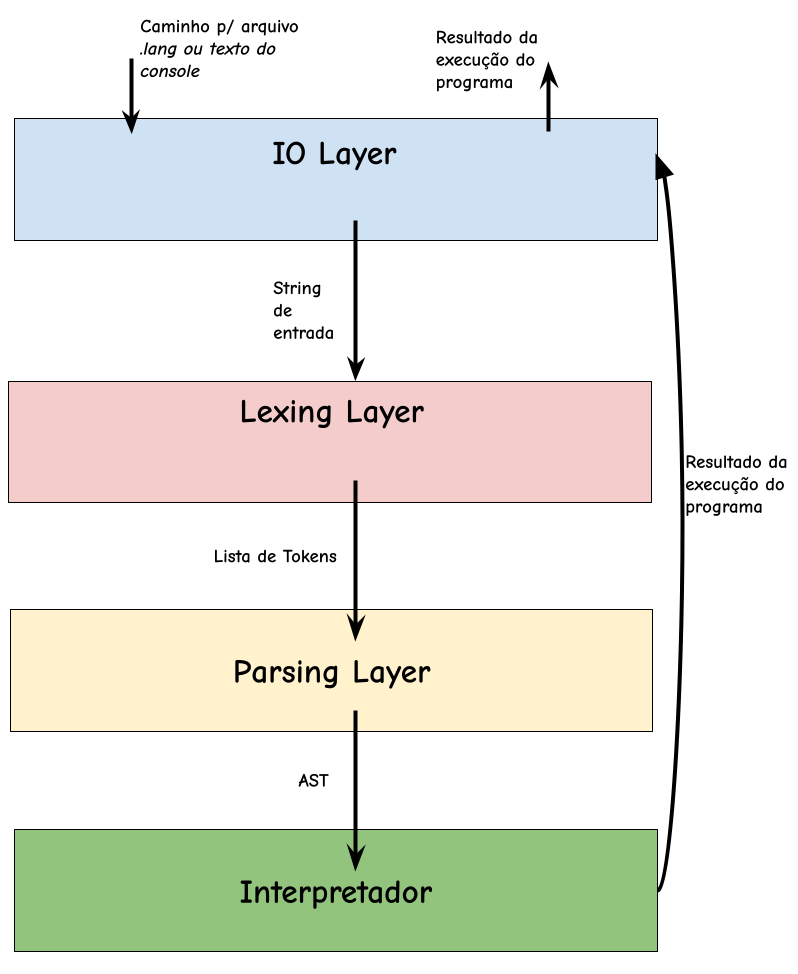
\includegraphics[width=13cm]{architecture-compiladores.png}
\caption{Arquitetura do projeto}
\end{figure}

\newpage


\end{document}
